\section*{The Discrete Fourier Transform}

\subsection*{The DFT Equation}

We now have all the necessary knowledge to understand how the Discrete Fourier Transform works.  Here is the
equation for it below:

\begin{equation}
\label{eq:dft}
X_k = \sum_{n = 0}^{N - 1}x[n] \cdot e^{-i\frac{2\pi}{N}kn}
\end{equation}

There is a lot to unpack here.  At a high level $X_k$ represents how much of some frequency we have in
some signal $x[n]$.  $X_k$ is a complex number and is the result of the inner product of our signal $x[n]$
and some test frequency denoted by the complex exponential $e^{i\frac{2\pi}{N}kn}$.  If $X_k$ is zero, then
we know we do not have that frequency in $x[n]$.  If $X_k$ is non-zero, then we do have some amount of 
that frequency in $x[n]$.  The DFT equation is simply a mathematical description of the procedure described 
in Figure \ref{fig:testComplex}.  Though Equation \ref{eq:dft} may look daunting, its simply calculating the
inner product of two signals just as we have done before.

Noticeably absent though from Equation \ref{eq:dft} is any mention of frequency, usually described with the
variable $f$.  Understand that the DFT is in fact calculating the inner product of the signal $x[n]$ with some
 frequency.  However, we cannot determine what the frequency is without knowing the sampling rate.  This is
 true if we were to look at any sequence of samples including those operated on by the DFT.
If we were to simply look at a sequence of samples, say from just a simple sinusoid, we cannot make any
claims about the frequency of that sinusoid.  We need to know how fast those samples will be played back.  
 The faster the playback, then the higher the frequency.  Similarly, the slower the playback, then the lower
 the frequency.  Frequency can only be determined by the combination 
 of a sequence of samples in conjunction with a sampling rate, usually described as $f_s$.  With the DFT, we
 make no assumptions about the sampling rate of the signal $x[n]$.  We treat $x[n]$ as just a sequence of
 samples and we test every sinusoid that could be periodic along that sequence of samples.

Remember that our conditions for orthogonality only hold when we deal with two sinusoids that are periodic
 over some interval.
In the DFT, that interval is the number of samples of our audio signal $x[n]$ denoted by $N$. 
 A sinusoid is periodic along some interval if it competes an integer number
of cycles.  To test all the sinusoids that are periodic along $N$, we need to calculate the inner product with
the sinusoids that evenly complete one cycle, two cycles, three cycles, four cycles, etc.   The variable $k$ denotes
the number of complete cycles that our testing sinusoid completes.  If we know the sample rate $f_s$, we
can determine the frequency of the sinusoid we are testing using $k$ and $N$.  The sample rate is a ratio of
the number of samples taken per second.  If we divide the sample rate by $N$, we can calculate how many 
periods of $N$ it takes to span one second of time.  For example if $f_s = 1000$Hz and $N = 250$, then
$f_s/N = 4$ tells us that four cycles of $N$ constitutes one second of time.  If we know that our testing sinusoid
completes $k$ cycles over those $N$ samples, then it must complete $k \cdot f_s/N$ across one second which is
simply the frequency of the sinusoid.  Therefore, we can state that $f = \frac{k}{N}f_s$.  Therefore, we know the
frequency represented by $X_k$ once we have the sampling rate.  In fact, you can see in the complex sinusoid
all the components for determing frequency (i.e., $\frac{k}{N}$) except the sampling rate.  So the DFT does in
fact encode all the information for the frequency of the test sinusoid once the sample rate as known.  
	
	Perhaps
you may be wondering why the sample rate is simply not included in the DFT equation.  That's a reasonable 
question and would make sense in the domain of audio.  In fact, we could write a variation of the DFT equation
that takes into account the sample rate of our signal.

\begin{equation}
\label{eq:dftFS}
	X_f = \sum_{n = 0}^{N - 1}x[n] \cdot e^{-i2\pi \frac{f}{f_s}n}
\end{equation}

Here we take the same inner product of $x[n]$ with some complex sinusoid of frequency $f$ and known sample
rate $f_s$.  It is easy to see that this new variation is equivalent to Equation \ref{eq:dft} by the fact that 
$f = \frac{k}{N}f_s$.  However, if you were to use the version of the DFT from Equation \ref{eq:dftFS}, you
would need to be sure that the frequencies you tested were in fact periodic along the interval $N$.  While Equation
\ref{eq:dftFS} may translate the standard DFT equation to the variables of $f$ and $f_s$ that you are likely
more comfortable with, it becomes much less obvious what frequencies actually do complete integer number
of cycles along $N$.  That is the purpose of the variable $k$ and why Equation \ref{eq:dft} is actually the easier
way to view the computation of the DFT.  It is also very little work to figure out the frequency with 
$f = \frac{k}{N}f_s$.

Below summarizes the meaning of each variable in the DFT equation.

\begin{itemize}
	\item $x[n]$: the signal
	\item $n$: the indexing variable
	\item $X_k$: a complex number that is the result of the inner product of $x[n]$ and a complex sinusoid
	\item $k$: the number of complete cycles our testing complex sinusoid completes
	\item $N$: the number of samples of our signal $x[n]$
	\item Frequency can be determined if the sampling rate is known by using $f = \frac{k}{N}f_s$
\end{itemize}

\subsection*{A Simple Example}

Let's use a simple example to illustrate how to use the DFT equation.  Let us take a very small example.  Suppose
we have samples drawn from the following signal $x = 0.5\cos(2\pi t + \pi) + 0.25\cos(4\pi t - 1)$.  The signal
$x$ contains two sinusoids of frequency 1Hz and 2Hz with differing phases and amplitudes.  Let us say we
were to draw eight samples ($N = 8$) from $x$ at a sampling rate of 8Hz for ease.  Here are those samples below:

$$x[n] = [-0.3649, -0.1432, -0.1351, 0.1432, 0.6351, 0.5639, -0.1351, -0.5639]$$

Now let us use the DFT equation to check whether to see our sampled signal contains the frequency 2Hz.  We 
of course know that it does but the DFT should give us a non-zero value.  Let us verify that is in fact true.  We
need to first figure out what $k$ should be.  We can simply solve using $f = \frac{k}{N}f_s$ and determine that
for $f = 2$, we should use $k = 2$.  Plugging in our values for $k$ and $N$, we now need to compute the following:

$$X_2 = \sum_{n = 0}^{7}x[n] \cdot e^{-i\frac{\pi}{2}n}$$

Unfortunately, we cannot just simply plug this into our normal calculators and figure out what $X_2$ is.  The complex exponential needs to be converted into its sinusoidal form using Euler's formula as shown in Equation
 \ref{eq:euler} in order to be calculated.  So let us rewrite that now:

$$X_2 = \sum_{n = 0}^{7}x[n] \cdot (\cos{(-\frac{\pi}{2}n)} +  i\sin(-\frac{\pi}{2}n)) = 
\sum_{n = 0}^{7}x[n]\cos{(-\frac{\pi}{2}n)} + i\sum_{n = 0}^{7}x[n]\sin(-\frac{\pi}{2}n))$$

Let us calculate each summation independently.  The left summation is the real part of the complex number $X_2$
and the right summation is the imaginary part.  

\begin{align*}
	\sum_{n = 0}^{7}x[n]\cos{(-\frac{\pi}{2}n)} =  & (x[0] \cdot 1) + (x[1] \cdot 0) + (x[2] \cdot -1) + (x[3] \cdot 0)\\
	& + (x[4] \cdot 1) + (x[5] \cdot 0) + (x[6] \cdot -1) + (x[7] \cdot 0)\\
	=  & x[0] - x[2] + x[4] - x[6] \\
	=  & -0.3649 - (-0.1351) + 0.6351 - (-0.1351) \\
	= & 0.5404
\end{align*}

Half of the result trivially goes away because many of those samples are multiplied by zero.  The bracket notation
$x[1]$, for example, simply means to use the 1st sample from $x[n]$.  Note that we count starting from index 0
in this notation so $x[1] = -0.1432$ and not -0.3649.  Using the same procedure, we can calculate
the imaginary summation as well and we will see that the result is $-0.8415i$.  Therefore, the value of 
$X_2$ is $0.5404 - 0.8415i$.  Note that $X_2$ is non-zero!  Therefore we can see that the frequency 2Hz is
indeed part of our signal as it should be.

If we want to test whether 3Hz is a part of $x[n]$, then we can calculate the DFT with the appropriate $k$ for
3Hz which also happens to be 3.  Using the same procedure, we would find that $X_3 = 0 + 0i$.  $X_3$ is
zero, meaning that 3Hz is not part of $x[n]$ as expected.  Of course, we will almost always be using the
DFT on unknown signals for $x[n]$.  The DFT can let us test to see whether a periodic sinusoid is part of our
signal.

\subsection*{Reconstructing Magnitude and Phase}

While the DFT can tell us whether a certain frequency is part of some signal, it can do even better.  The complex
number $X_k$ can be used to reconstruct the magnitude and phase of the sinusoid as well.  Let us assume that
the signal $x[n]$ has a sinusoid of the form $A\cos(2\pi f Tn + \phi)$ \footnote{We could very well assumed a sinusoid of the form $A\sin(2\pi fTN + \phi)$ instead of using a 
cosine.  It certainly makes no mathematical difference as a sine wave and cosine wave are only differentiated
by their phase.  It will be nicer mathematically if we think about it as a cosine wave.  The corresponding
$X_k$ would have a complex number of the form $	X_k = \frac{AN\sin(\phi)}{2} - \frac{AN\cos(\phi)}{2}i$. While this is perfectly valid, the careful reader will note that the angle or argument of the complex number
does not match $\phi$ as it does in the cosine form.  The cosine form presents a nice convenience.} that is periodic along the interval $N$.  
If it is periodic along $N$, we can also write the sinusoid in the form $A\cos(2 \pi \frac{k}{N} n + \phi)$.  The
latter form matches nicely with $X_k$ because the subscript $k$ from $X_k$ is the same $k$ in 
$A\cos(2 \pi \frac{k}{N} n + \phi)$.  When we take the DFT for $x[n]$,  the complex number will be of the form
shown in Equation \ref{eq:complexNumber} if the sinusoid exists in $x[n]$.  Remember it will be 0 otherwise.

\begin{equation}
	\label{eq:complexNumber}
	X_k = \frac{AN\cos(\phi)}{2} + \frac{AN\sin(\phi)}{2}i
\end{equation}

 In some notations for complex numbers, the real part and imaginary parts of a complex number is 
 given with the symbols: $\RE()$ and $\IM()$, respectively.  If I had an imaginary number $z = 3 + 4i$, then
 $\RE(z) = 3$ and $\IM(z) = 4$.  The symbols themselve may seem complex but they are
 simply a convenience for referring to the two components of an imaginary number.  Therefore, I could say
 that in our particular example with $x[n]$ that $\RE(X_k) = \frac{AN\cos(\phi)}{2}$ and $\IM(X_k) = 
 \frac{AN\sin(\phi)}{2}$.  Given Equation \ref{eq:complexNumber} and our handy tools for referring to the
 imaginary and real parts of a complex number, we can derive the amplitude $A$ from $X_k$ as follows:


\begin{equation}
\label{eq:amplitude}
	A = \frac{2}{N}\sqrt{(\RE(X_k))^2 + (\IM(X_k))^2}
\end{equation}

Recalling our example above, let's reconstruct the magnitude from $X_2 = 0.5404 - 0.8415$.  Plugging in 
the real and imaginary component to Equation \ref{eq:amplitude}, we get 
$A = \frac{2}{8}\sqrt{(0.5404)^2 + (-0.8415)^2} = 0.25$.  If we look back at the original signal $x =
0.5\cos(2\pi t + \pi) + 0.25\sin(4\pi t - 1)$, you will see that the sinusoid with frequency 2Hz does indeed
have an amplitude of 0.25.  

Similarly, we can also use $X_k$ to get back the phase $\phi$ of the sinusoid as well.  Equation \ref{eq:phase}
shows the formula for doing so.

\begin{equation}
\label{eq:phase}
\phi = \tan^{-1}\bigg(\frac{\IM{(X_k)}}{\RE{(X_k)}}\bigg)
\end{equation}

From the same example, if we compute $\tan^{-1}(\frac{-0.8415}{0.5404})$, we get -1 which is indeed the
phase of $0.25\sin(4\pi t - 1)$.  One needs to be careful when using the inverse tan function with computers
or calculators.  The sign of the real and imaginary part indicates which quadrant the phase will be located.  Most
computers and calculators however keep the phase between $-\frac{\pi}{2}$ and $\frac{\pi}{2}$.  Some software
like Matlab and others offer a special function that takes into the account the sign of the numerator and denominator.  It is sometimes referred to as ``atan2" or ``arctan2".  It is fine to use either but you simply need
to be aware of the limitations of your software and may need to correct some phases by hand if your calculator
keeps the phase between $-\frac{\pi}{2}$ and $\frac{\pi}{2}$.

These two equations will work for nearly all the frequency bins $X_k$. The exceptions are when $k/N$
is a multiple of $\frac{1}{2}$ which corresponds to $k = N/2$ (i.e., the Nyquist frequency) and $k = 0$ 
(sometimes termed the D.C. offset).  In these 
instances, the complex number $X_k$ cannot be used to recover the original amplitude and phase because
$X_k = AN\cos{(\phi)} + 0i$.  Because the imaginary component is zero, we do not have a way to determine
what proportion of $A$ and $\phi$ contribute to the real component of $X_k$.  We simply have too many 
variables and not enough information.  Generally though, this is not a big deal.  We do not expect to have
any frequency component at the Nyquist frequency if we have properly filtered our signal to prevent aliasing.
The D.C. offset is also rather inconsequential.  D.C. offset refers to how far away the average of a signal
deviates from zero.  It is not a component of the signal that contributes to pitch.  

\subsection*{Frequency Bins}

The DFT equation from Equation \ref{eq:dft} only calculates the inner product of our signal against one
frequency.  Typically though we want to calculate the DFT for numerous frequencies.  Remember that
frequency is not explicitly stated in the DFT equation.  $k$ is the variable we use to test our signal against
different periodicities.  The DFT calculates all values of $k$ from 0 all the way up to $N - 1$.  A value of $k = 0$
calculates how much D.C. bias is in the signal (i.e., if the averages of the samples is something other than zero).
A value of $k = \frac{1}{2}N$ tests for presence of the Nyquist frequency defined as half the sampling rate.  
A value of $k = N$ would test for the 
presence of the frequency equal to the sampling rate $f_s$ but it turns out that the DFT starts repeating itself
starting at $k = N$.  You can test this yourself but $X_0 = X_N$ and $X_1 = X_{N + 1}$ and so on.

\begin{figure}[h]
	\caption{A table of the DFT results from samples of $0.5\cos(2\pi t + \pi) + 0.25\cos(4\pi t - 1)$}
	\label{fig:dftTable}
	\begin{center}
		\begin{tabular}{ |c|c|c|c|c|c|c| } 
			\hline
			k & Frequency (in Hz) & $X_k$ & $X_k$ Magnitude & $X_k$ Phase & Magnitude & Phase \\ 
			\hline
			0 & 0 & $0 + 0i$ & 0 & 0 & 0 & 0 \\ 
			1 & 1 & $-2 + 0i$ & 2 & $\pi$& 0.5 & $\pi$ \\
			2 & 2 & $0.5403 - 0.8415i$ & 1 & -1 &0.25 & -1 \\
			3 & 3 & $0 + 0i$ & 0 & 0 & 0 & 0 \\
			4 & 4 & $0 + 0i$ & 0 & 0 & 0 & 0 \\
			5 & 5 & $0 + 0i$ & 0 & 0 & 0 & 0 \\
			6 & 6 & $0.5403 + 0.8145i$ & 1 & 2.57 & 0.25 & $1$ \\
			7 & 7 & $-2 + 0i$ & 2 & $-\pi$ & 0.5 & $-\pi$ \\
			\hline
		\end{tabular}
	\end{center}
	
\end{figure}

Figure \ref{fig:dftTable} shows a table of all the calculations from the DFT in the column labeled $X_k$.  For
convenience, the frequency of each bin is also given.  Because the number of samples equals the sampling rate,
the value of $k$ is in fact the frequency but that will rarely be the case.  We generally deal with very high
sampling rates like 44.1kHz and smaller numbers of samples for the DFT.  To calculate the frequency of each
$X_k$, sometimes referred to as frequency bins, we simply compute $k\frac{f_s}{N}$.  You can see that in
our trivial example that $\frac{f_s}{N} = \frac{8}{8} = 1$ so the frequency of each bin is just $k$.

	The magnitude and phase for
each complex number $X_k$ are given.  See Appendix A for more information about how the magnitude and phase
are calculated for a complex number.  Generally, when we examines plots of the DFT, we are looking at graphs
of the magnitude and phase of the complex number.  The magnitude of $X_k$ tells us how much of that frequency
 is present in the original signal.  The magnitude of $X_k$ is proportional to the amplitude of 
 the original frequency, but it does not give the exact amplitude of the original frequency.  
 For that we would need to use Equation \ref{eq:amplitude}.  The original phase and the phase of the complex 
 number are also given as well.  For music applications, the phase is usually unimportant
 information.  We generally care most about the magnitude because small differences in phase tend to not
 impact the way we perceive sound.  There are exceptions though and in some applications we need to be 
 careful with the way we treat phase.

\subsection*{Interpreting Magnitude and Phase Graphs}

When we perform the DFT on a particular signal, we often display the magnitude and phase graphically.  Below
are two examples of the magnitude and phase spectrum of some signal $x[n]$ with sample rate $f_s = 256$Hz and
$N = 128$.  Let's see what we can
deduce about the time domain form of the signal from these two spectrums.

\begin{figure}[h]
	\caption{The magnitude spectrum of $x[n]$ at $f_s = 256$ and $N = 128$}
	\label{fig:magnitudeGraph}
	\begin{center}
	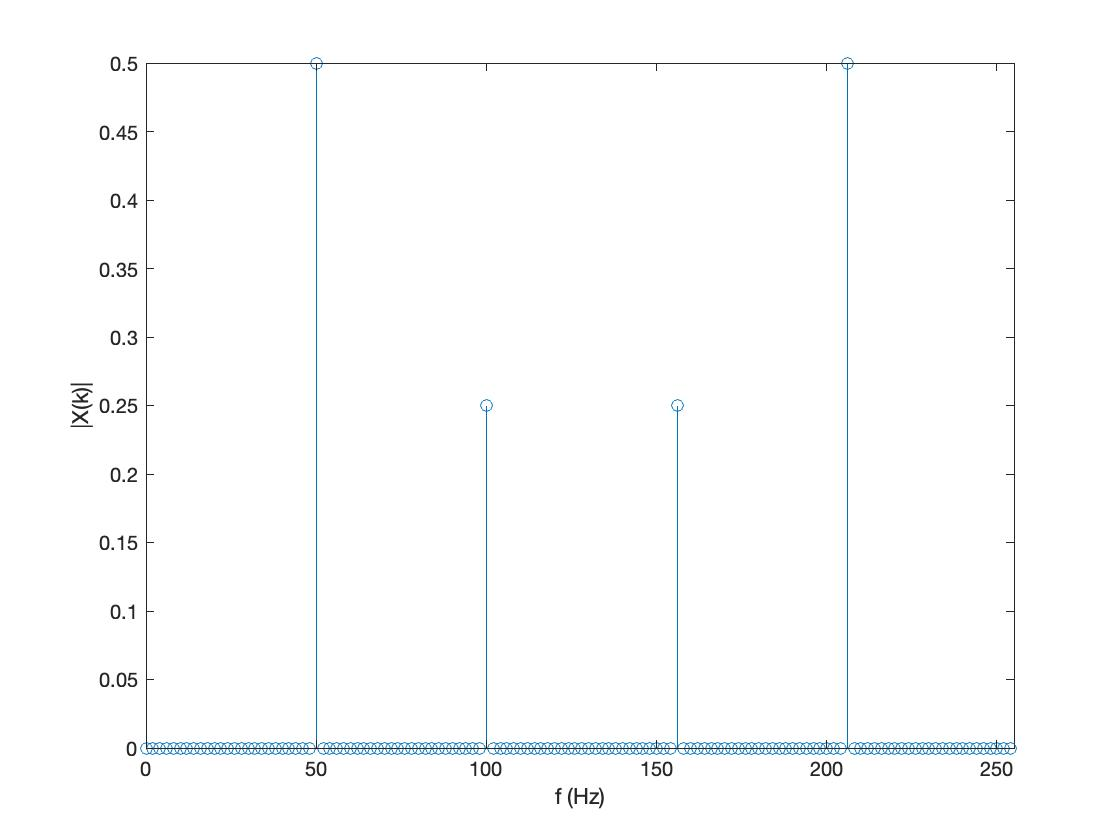
\includegraphics[scale = 0.3]{magnitude.jpg}
	\end{center}
\end{figure}

\begin{figure}[h]
	\caption{The phase spectrum of $x[n]$ at $f_s = 256$ and $N = 128$}
	\label{fig:phaseGraph}
	\begin{center}
		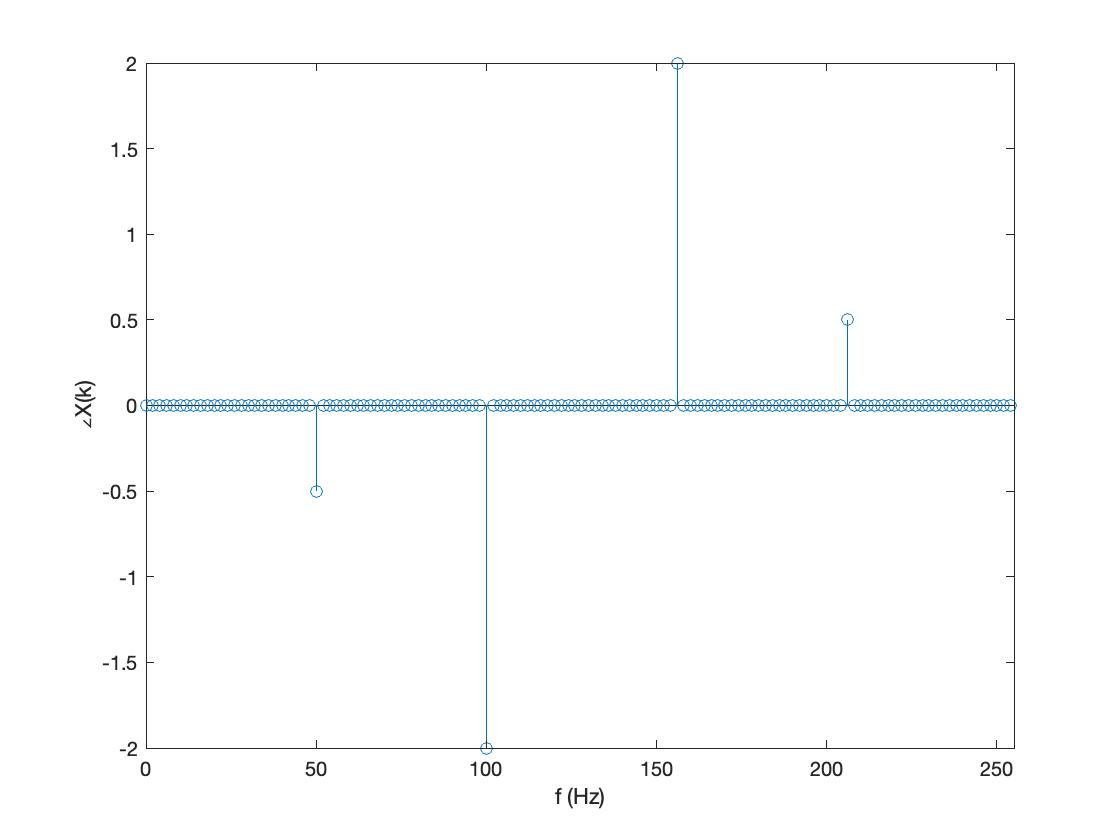
\includegraphics[scale = 0.3]{phase.jpg}
	\end{center}
\end{figure}

Figure \ref{fig:magnitudeGraph} shows the magnitude spectrum of $x[n]$.  When looking at the magnitude 
spectrum of a sound it is important to know how the magnitude is scaled.  The magnitude of a complex number
is always calculated as $\sqrt{(\RE{(z)})^2 + (\IM{(z)})^2}$; however, that magnitude is sometimes multiplied by
a constant.   An unnormalized magnitude simply computes $\sqrt{(\RE{(z)})^2 + (\IM{(z)})^2}$.  
Plotting unnormalized magnitudes is less common.  Why?  The magnitude spectrum is proportional to the size
of $N$.  A larger number of samples $N$ will proportionally increase the magnitude spectrum of the signal 
even if there is no change in the sinusoidal components of the signal.  Look back at Equation \ref{eq:complexNumber}.  You will see that $X_k$ can increase or decrease without change to $A$ or $\phi$
simply by changing $N$.  An altenative is to simply divide out the factor of $N$, and sometimes the factor of 
$1/2$, from the real and imaginary
component so that the value of each frequency bin is related solely by the phase and amplitude of the original
sinusoidal component.  This is referred to as a normalized magnitude spectrum.  The normalized
magnitude spectrum is calculated as $\frac{1}{N}\sqrt{(\RE{(z)})^2 + (\IM{(z)})^2}$.  

	Figure \ref{fig:magnitudeGraph} shows the normalized magnitude spectrum as 
$\frac{2}{N}\sqrt{(\RE{(z)})^2 + (\IM{(z)})^2}$ to remove the factor of $1/2$.  This is exactly equivalent to
Equation \ref{eq:amplitude}.  Therefore, the advantage here is that 
the magnitude spectrum of Figure \ref{fig:magnitudeGraph} depicts the exact amplitude of each sinusoidal
component of the original signal.  In general though, the magnitude is usually calculated as 
$\frac{1}{N}\sqrt{(\RE{(z)})^2 + (\IM{(z)})^2}$.  The form of $\frac{2}{N}\sqrt{(\RE{(z)})^2 + (\IM{(z)})^2}$ is
ideal if we know that all frequency components of $x[n]$ are periodic along $N$.  This assumption about
periodicity is the key for asserting Equation \ref{eq:complexNumber}.  Most signals, however, will not
be perfectly periodic along $N$.  In fact, the DFT will not allow us to perfectly reconstruct the exact frequencies,
amplitudes, and phases using the complex frequency bins if the signal has aperiodic frequency components
along $N$.  Therefore, we usually just see the normalized magnitude spectrum in the form of 
$\frac{1}{N}\sqrt{(\RE{(z)})^2 + (\IM{(z)})^2}$ or the unnormalized form.

Let us examine Figure \ref{fig:magnitudeGraph}.  We see four peaks in the graph.  The magnitude spectrum
here is calculated using $\frac{2}{N}\sqrt{(\RE{(z)})^2 + (\IM{(z)})^2}$, equivalent to the amplitude of each
sinusoidal component.  Therefore, we see four amplitudes at frequencies 50Hz, 100Hz, 156Hz, and 206Hz.  
We can ignore the components of the spectrum above the Nyquist frequency of 128Hz.  Therefore, we have two
sinusoidal components in $x[n]$: 50Hz at an amplitude of 0.5 and 100Hz at an amplitude of 0.25.  

Note the symmetry in the magnitude spectrum.  If we were to draw a straight line down the center of the 
magnitude spectrum at the Nyquist frequency, the left half and right half would be perfectly symmetrical.  
A fundamental property of the DFT is that when $x[n]$ is a real signal and does not include any complex
components, the two halves of the DFT are symmetrical.  Because we are dealing solely with audio signals,
we always use the DFT with real signals and therefore will always have symmetry.  

Figure \ref{fig:phaseGraph} shows the phase spectrum of $x[n]$.  The phase spectrum of a signal depicts
the argument or phase of the complex number $X_k$.  Recall that the argument of the complex number is 
the angle
between the imaginary and real components if we were to plot them on a 2D graph.  Why plot the argument
of the complex number?  The phase of the original sinusoidal
component is exactly the argument of the complex number, assuming we model the sinusoidal component 
as a cosine wave.  As expected we see peaks at exactly 50Hz, 100Hz, 156Hz, and 206Hz.  Again, we can 
ignore the two frequencies above the Nyquist frequency.  We can see phases of $-0.5$ and $-2$ at 50Hz and 
100Hz, respectively.  Putting together the information from the magnitude and
phase spectrum, we can perfectly recreate the original signal: 
$x[n] = 0.5\cos(2\pi(50)t - 0.5) + 0.25\cos(2\pi(100)t - 2)$.

There is also symmetry in the phase spectrum as well.  Again if we were to draw a straight line vertically at
the Nyquist frequency and flip the signs of one of the halves, we would have two symmetrical halves.  Again
these symmetrical properties are true for all real signals $x[n]$ such as audio.
